\documentclass[12pt]{article}

\usepackage[margin=0.8 in]{geometry}
\usepackage{amsmath}
\usepackage{amssymb}
\usepackage{mathtools}
\usepackage{enumerate}
\usepackage{verbatim}
\usepackage{amsthm}
\usepackage{hyperref}

\title{}
%\content{}



\let \proj \undefined
\newcommand{\p}{\partial}
\newcommand{\R}{ \mathbb{R}}

\DeclareMathOperator{\proj}{proj}
\newcommand{\sS}{\mathscr{S}}
\DeclareMathOperator{\comp}{comp}
\newcommand{\A}{\mathcal{A}}
\newcommand{\D}{\mathcal{D}}
\newcommand{\e}{\epsilon}
\newcommand{\et}{\tilde{\e}}
\newcommand{\vr}{\vec{r}{}}
\newcommand{\vF}{\vec{F}}
\newcommand{\triple}{\iiint_E f(x,y,z)dV}
\renewcommand{\lg}{\langle}
\newcommand{\rg}{\rangle}
\newcommand{\Q}{\frac{\p Q}{\p x}}
\renewcommand{\P}{\frac{\p P}{\p y}}
\let\implies\Rightarrow
\newcommand{\n}{\nabla}
\newcommand{\Fline}{\vF\cdot d\vr}
\newcommand{\vi}{\vec{i}}
\newcommand{\vj}{\vec{j}}
\newcommand{\vk}{\vec{k}}
\DeclareMathOperator{\curl}{curl}

\newcommand{\rcross}{\vr_u\times\vr_v} 
\newcommand{\Fsur}{\vF\cdot d\vS}
\newcommand{\vn}{\vec{n}}
\newcommand{\vS}{\vec{S}}
\newcommand{\flux}{\iint_S \vF\cdot d\vS}
\newcommand{\vG}{\vec{G}}
\let \div \undefined
\DeclareMathOperator{\div}{div}



\newenvironment{solution}
  {\begin{proof}[Solution]}
  {\end{proof}
  
  }
\newtheorem{example}{Example}
\newtheorem{exercise}{Exercise}
\newtheorem{theorem}{Theorem}
\newtheorem{defn}{Definition}


\begin{document}
\section*{The Divergence Theorem}

In the last section we saw a theorem about closed curves. In this one we'll see a theorem about closed surfaces (you can imagine bubbles). As we've mentioned before, closed surfaces split $\R^3$ two domains, one bounded and one unbounded.


\begin{theorem}(Divergence)
Suppose we have a \textbf{closed} parametric surface with \textbf{outward orientation } that is the boundary of the bounded domain $E$ in $\R^3$. Also, let $\vF$ be a vector field in $\R^3$ with differentiable coefficients. Then
$$\iint_S\Fsur=\iiint_E \div \vF dV.$$
\end{theorem}

\textbf{Remarks:}
\begin{enumerate}
\item It is very important that it is a \textbf{closed} surface that we're finding the flux of $\vF$ across. To understand this, find the flaw in the following argument:

``Let $c$ be a simple closed curve in $\R^3$ and $\vF$ be a vector field. Then:
$$\int_c \Fline \overset{\mathrm{Stokes}}{=}\iint_S \curl \vF\cdot d\vS\overset{\mathrm{Divergence}}{=}\iiint_E \div\curl\vF dV=0,$$ since $\div\curl\vF=0$ for any vector field $\vF$, as we've already seen.''

\item As with Stokes' Theorem, we often denote the positively oriented boundary of a solid $E$ by $\p E$ and write the Divergence Theorem as $$\iint_{\p E}\Fsur=\iiint_E \div \vF dV.$$

\item If a closed surface $S$ that is the boudary of a domain $E$ is \textbf{negatively oriented}, we have $$\iint_S\Fsur=-\iiint_E \div \vF dV.$$

\item When is the divergence theorem useful? Usually whenever we would like to compute a flux across a closed surface, especially when the surface consists of several smooth smaller surfaces and we'd need to write a sum of integrals. See the following example:

\begin{example}
Find the flux $\flux$, where $\vF=\lg x,-1,2y\rg $ and $S$ is the positively oriented boundary of the solid $E$ in $\R^3$ bounded by the $xy$ plane, the cylinder $x^2+y^2=1$ and the plane $z=2-x$.
\end{example}

\begin{figure}[h]
\begin{center}
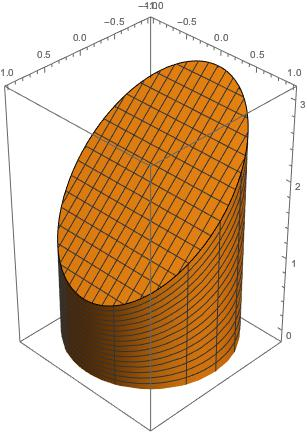
\includegraphics[scale=.3]{cylinder.jpeg}
\end{center}
\end{figure}
\begin{solution}
We could find the flux by computing three surface integrals, but it's easier to use the Divergence Theorem instead. We have:
$$\flux=\iiint_E \div\lg x,-1,2y\rg dV=\iiint_E 1 dV=\int_0^{2\pi}\int _0^1\int_0^{2-r\cos(\theta)}rdzdrd\theta$$
\end{solution}

Another situation where the divergence theorem can be useful is when we don't have a closed surface, but we can complete into a closed surface to make a computation easier.

Let's see an example:

\begin{example}
Compute the flux $\flux$, where $\vF=\lg x,-1,2y\rg $ and $S$ consists of the five sides other than the lower one of the cube $E$ with vertices (-1,-1,0), (1,-1,0), (1,1,0), (-1,1,0), (1,1,2), (-1,1,2), (1,-1,2), (-1,-1,2) and outward orienation.
\end{example}

\begin{figure}[h]
\begin{center}
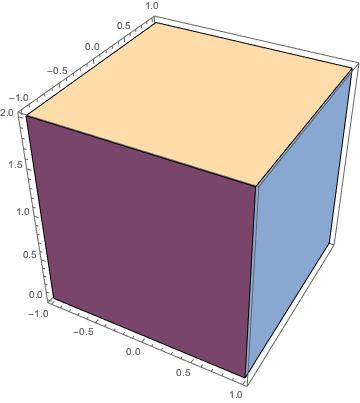
\includegraphics[scale=.3]{cube.jpeg}
\end{center}
\end{figure}

\begin{solution}
Normally we'd have to compute 5 surface integrals and add them. Note that this is \textbf{not} a closed surface, so we can't apply the Divergence Theorem directly. What we can do is attach an extra face to the cube with appropriate orientation and make into a closed surface. That is, we attach the face $S'$ parametrized as $$\vr(u,v)=\lg u,v,0\rg,\text{ for }(u,v)\in [-1,1]\times[-1,1].$$
We give it \textbf{downward} orientation, so that $S'\cup S$ ends up being a closed surface with outward orientation. Then, by Divergence theorem, $$\iint_{S\cup S'} \Fsur=\iiint_E\div \vF dV=\iiint_E 1 dV=2^3=8.$$

Since $$\flux=\iint_{S'\cup S}\Fsur-\iint_{S'}\Fsur,$$
we only need to compute $\iint_{S'}\Fsur$. Since $S'$ is a surface on the $xy$ plane with downward orientation, its unit normal vector field is $\vec{n}=-\lg 0,0,1\rg$ and we have $$\iint_{S'\cup S}\Fsur=\int_{-1}^1\int_{-1}^1 \lg u,-1, 2v\rg\cdot\lg 0,0,-1\rg dudv=0 $$ and so $$\flux=8.$$

\end{solution}

\item What does the Divergence Theorem say from a physical point of view? When we discussed divergence, we said that divergence describes the extent to which the vector field behaves like a source (positive divergence) or as a sink (negative divergence) near a point $p$. Then, the Divergence Theorem roughly says that summing up all the infinitesimally small sources and subtracting all the sinks inside a domain of $\R^3$ gives the total flux on its boundary. 

\item The Divergence Theorem holds in any dimension, and in dimension 2 it is equivalent Green's Theorem (this means that you can derive it from Green's Theorem and you can derive Green's Theorem from the Divergence Theorem).



\end{enumerate}


\subsection*{Green's First Identity}

We can use use the Divergece Theorem to derive the following useful formula. Let $E$ be a domain in $\R^3$ and $\p E$ its positively oriented boundary with unit normal $\vec{n}$. Then, if $u$, $v$ are twice differentiable scalar valued functions, we have $$\iint_{\p E} vD_{\vn}u-u D_{\vn}vdS=\iiint_Ev\Delta u-u\Delta vdV.$$

We have \begin{align}
\div(u\n v)=&\p_x(u\p_xv)+\p_y(u\p_yv)+\p_z(u\p_zv)\\
=&\p_xu\p_xv+\p_yu\p_yv+\p_zu\p_zv+u(\p^2_xv+\p^2_yv+\p^2_zv)\\
=&\nabla u\cdot\n v+u\Delta v\label{eq1}
\end{align}
Similarly, \begin{equation}
\div(v\n u)=\n v\cdot\n u+v\Delta u\label{eq2}
\end{equation}
Subtract \eqref{eq1} from \eqref{eq2} and find $$\div(v\n u-u\n v)=v\Delta u-u\Delta v.$$ Then e integrate over $E$ and use Divergence Theorem:
\begin{align*}
\iiint_E v\Delta u-u\Delta v dV=&\iiint_E \div(v\n u-u\n v)dV\\
=& \iint_{\p E} (v\n u-u\n v)\cdot d\vS\\
=& \iint_{\p E} (v\n u-u\n v)\cdot\vn dS\\
=& \iint_{\p E} vD_{\vn}u-u D_{\vn}vdS
\end{align*}
\end{document}

